\documentclass[modern]{aastex62}

\pdfoutput=1

%\usepackage{lmodern}
%\usepackage{microtype}
\usepackage{url}
\usepackage{amsmath}
\usepackage{amssymb}
\usepackage{natbib}
\usepackage{multirow}
\usepackage{graphicx}
\bibliographystyle{aasjournal}

\usepackage{mathtools}
\usepackage{calc}
\usepackage{etoolbox}
\usepackage{xspace}
\usepackage[T1]{fontenc} % https://tex.stackexchange.com/a/166791
\usepackage{textcomp}
\usepackage{ifxetex}
\ifxetex
\usepackage{fontspec}
\defaultfontfeatures{Extension = .otf}
\fi
\usepackage{fontawesome}

% Matrix fix:
% http://tex.stackexchange.com/questions/317824/letter-c-appearing-inside-pmatrix-environment-with-aastex
\makeatletter
\def\env@matrix{\hskip -\arraycolsep\let\@ifnextchar\new@ifnextchar\array{*{\c@MaxMatrixCols}c}}
\makeatother

% Column spacing in matrix
% http://tex.stackexchange.com/questions/275725/adjusting-separation-between-matrix-entries
\setlength\arraycolsep{25pt}

% ------------------ %
% end of AASTeX mods %
% ------------------ %

% Projects:
\newcommand{\project}[1]{\textsf{#1}}
\newcommand{\exoplanet}{\project{exoplanet}}
\newcommand{\starry}{\project{starry}}
\newcommand{\radvel}{\project{RadVel}}
\newcommand{\batman}{\project{batman}}
\newcommand{\python}{\project{Python}}
\newcommand{\cython}{\project{Cython}}
\newcommand{\cpp}{\project{C++}}
\newcommand{\theano}{\project{Theano}}
\newcommand{\pymc}{\project{PyMC3}}
\newcommand{\pytorch}{\project{PyTorch}}
\newcommand{\tensorflow}{\project{TensorFlow}}
\newcommand{\stan}{\project{Stan}}
\newcommand{\celerite}{\project{celerite}}
\newcommand{\tess}{\project{TESS}}


% references to text content
\newcommand{\documentname}{\textsl{Note}}
\newcommand{\figureref}[1]{\ref{fig:#1}}
\newcommand{\Figure}[1]{Figure~\figureref{#1}}
\newcommand{\figurelabel}[1]{\label{fig:#1}}
\renewcommand{\eqref}[1]{\ref{eq:#1}}
\newcommand{\Eq}[1]{Equation~(\eqref{#1})}
\newcommand{\eq}[1]{\Eq{#1}}
\newcommand{\eqalt}[1]{Equation~\eqref{#1}}
\newcommand{\eqlabel}[1]{\label{eq:#1}}

% TODOs
\newcommand{\todo}[3]{{\color{#2}\emph{#1}: #3}}
\newcommand{\dfmtodo}[1]{\todo{DFM}{red}{#1}}
\newcommand{\alltodo}[1]{\todo{TEAM}{red}{#1}}
\newcommand{\citeme}{{\color{red}(citation needed)}}

% math
\newcommand{\T}{\ensuremath{\mathrm{T}}}
\newcommand{\dd}{\ensuremath{ \mathrm{d}}}
\newcommand{\unit}[1]{{\ensuremath{ \mathrm{#1}}}}
\newcommand{\bvec}[1]{{\ensuremath{\boldsymbol{#1}}}}

% typography obsessions
\setlength{\parindent}{3.0ex}

% from: https://github.com/rodluger/corTeX
% Add code, proof, and animation hyperlinks
\definecolor{linkcolor}{rgb}{0.1216,0.4667,0.7059}
\newcommand{\codeicon}{{\color{linkcolor}\faFileCodeO}}
\newcommand{\prooficon}{{\color{linkcolor}\faPencilSquareO}}
\newcommand{\codelink}[1]{\href{https://github.com/dfm/exoplanet/blob/3f5ce20d413f052d603c156162e3d0b95204367c/paper/figures/#1.ipynb}{\codeicon}\,\,}
\newcommand{\animlink}[1]{\href{https://github.com/dfm/exoplanet/blob/3f5ce20d413f052d603c156162e3d0b95204367c/paper/figures/#1.gif}{\animicon}\,\,}
\newcommand{\prooflink}[1]{\href{https://github.com/dfm/exoplanet/blob/3f5ce20d413f052d603c156162e3d0b95204367c/paper/proofs/#1.ipynb}{\raisebox{-0.1em}{\prooficon}}}


% Define a proof environment for open source equation proofs
\newtagform{eqtag}[]{(}{)}
\newcommand{\currentlabel}{None}
\newenvironment{proof}[1]{%
\ifstrempty{#1}{%
\renewtagform{eqtag}[]{\raisebox{-0.1em}{{\color{red}\faPencilSquareO}}\,(}{)}%
}{%
\renewtagform{eqtag}[]{\prooflink{#1}\,(}{)}%
}%
\usetagform{eqtag}%
\renewcommand{\currentlabel}{#1}
\align%
}{%
\endalign%
\renewtagform{eqtag}[]{(}{)}%
\usetagform{eqtag}%
\message{<<<\currentlabel: \theequation>>>}%
}

% Define the `oscaption` command for open source figure captions
\newcommand{\oscaption}[2]{\caption{#2 \codelink{#1}}}

\newcommand{\Gaussian}[3]{\ensuremath{\frac{1}{|2\pi #2|^\frac{1}{2}}
            \exp\left[ -\frac{1}{2}#1^\top #2^{-1} #1 \right]}}

\newcommand{\Normal}{\ensuremath{\mathcal{N}}}
\newcommand{\mA}{\ensuremath{\bvec{A}}}
\newcommand{\mC}{\ensuremath{\bvec{C}}}
\newcommand{\mS}{\ensuremath{\bvec{\Sigma}}}
\newcommand{\mL}{\ensuremath{\bvec{\Lambda}}}
\newcommand{\vw}{\ensuremath{\bvec{w}}}
\newcommand{\vy}{\ensuremath{\bvec{y}}}
\newcommand{\vt}{\ensuremath{\bvec{\theta}}}
\newcommand{\vm}{\ensuremath{\bvec{\mu}(\bvec{\theta})}}
\newcommand{\vre}{\ensuremath{\bvec{r}}}
\newcommand{\vh}{\ensuremath{\bvec{h}}}
\newcommand{\vk}{\ensuremath{\bvec{k}}}


\begin{document}\raggedbottom\sloppy\sloppypar\frenchspacing

\title{%
{\bf NOTE: this is a very rough draft of this manuscript --- read at your own risk!}
\\
\project{exoplanet}:
A toolkit for scalable inference for exoplanetary systems using transits,
radial velocities, \& astrometry
%An efficient and robust toolkit for gradient-based
%probabilistic characterization of exoplanets using transits and radial
%velocities
}

\author[0000-0002-9328-5652]{Daniel Foreman-Mackey}
\affil{Center for Computational Astrophysics, Flatiron Institute, 162 5th Ave, New York, NY 10010}

\author[0000-0002-1483-8811]{Ian Czekala}
\altaffiliation{NASA Hubble Fellowship Program Sagan Fellow}
\affiliation{Department of Astronomy, 501 Campbell Hall, University of California, Berkeley, CA 94720}

\author[0000-0002-0802-9145]{Eric Agol}\altaffiliation{Guggenheim Fellow}
\affil{Department~of~Astronomy, University~of~Washington, Seattle, WA 98195}
\affil{Virtual~Planetary~Laboratory, University~of~Washington, Seattle, WA 98195}

\author[0000-0002-0296-3826]{Rodrigo Luger}
\affil{Center for Computational Astrophysics, Flatiron Institute, 162 5th Ave, New York, NY 10010}

\begin{abstract}

As larger and more precise datasets continue to be collected for the discovery and characterization of exoplanets, we must also develop computationally efficient and rigorous methods for making inferences based on these data.
The efficiency and robustness of numerical methods for probabilistic inference
can be improved by using derivatives of the model with respect to the
parameters.
In this paper, I derive methods for exploiting these gradient-based methods
when fitting exoplanet data based on radial velocity, astrometry, and
transits.
Alongside the paper, I release an open source, well-tested, and
computationally efficient implementation of these methods.
These methods can substantially reduce the computational cost of fitting large
datasets and systems with more than one exoplanet.

\end{abstract}

\keywords{%
methods: data analysis ---
methods: statistical
}

\section{Outline}

\begin{enumerate}

{\item Introduction
\begin{itemize}
{\item the datasets available and forthcoming}
{\item existing tools for exoplanet fitting}
{\item motivation for gradients}
\end{itemize}}

\item Automatic differentiation and inference frameworks

\item Hamiltonian Monte Carlo and variants

\item Custom gradients required for exoplanet datasets
\begin{itemize}
\item Radial velocities and Kepler's equation
\item Astrometry
\item Transits
\end{itemize}

\item Implementation details and benchmarks

\item Examples

\item Discussion

\end{enumerate}

\section{Introduction}

Datasets are getting larger and more precise and this leads to an interest in
more ambitious questions about these systems.
The existing inference methods are no longer up to the task when the datasets
are large and when the number of parameters is large.
Many probabilistic inferences in astronomy have been limited by the existing
tools that can't scale e.g.\ emcee.
However, in other fields such as ML, methods have been developed that can
scale to datasets too large to fit into memory and millions of parameters.
The key ingredient in all of these methods is that it must be possible to
efficiently evaluate the derivative of the model with respect to the physical
parameters.
This can often be intractable for applications astrophysics because the models
generally include a physically motivated component that can't be trivially
differentiated.
However, we can take advantage of the substantial development that has been
invested in automating this process.

This paper presents an example of how these tools and methods can be
exploited in the specific astronomical application of fitting exoplanet
datasets.
We go through the derivation and implementation of the custom functions and
their gradients that are required for gradient-based characterization of
exoplanets.

These methods and their implementation are not an all-in-one package designed
to do the fitting.
Instead, it provided the framework needed to use these tools within pipelines.

\begin{figure}[htbp]
\begin{centering}
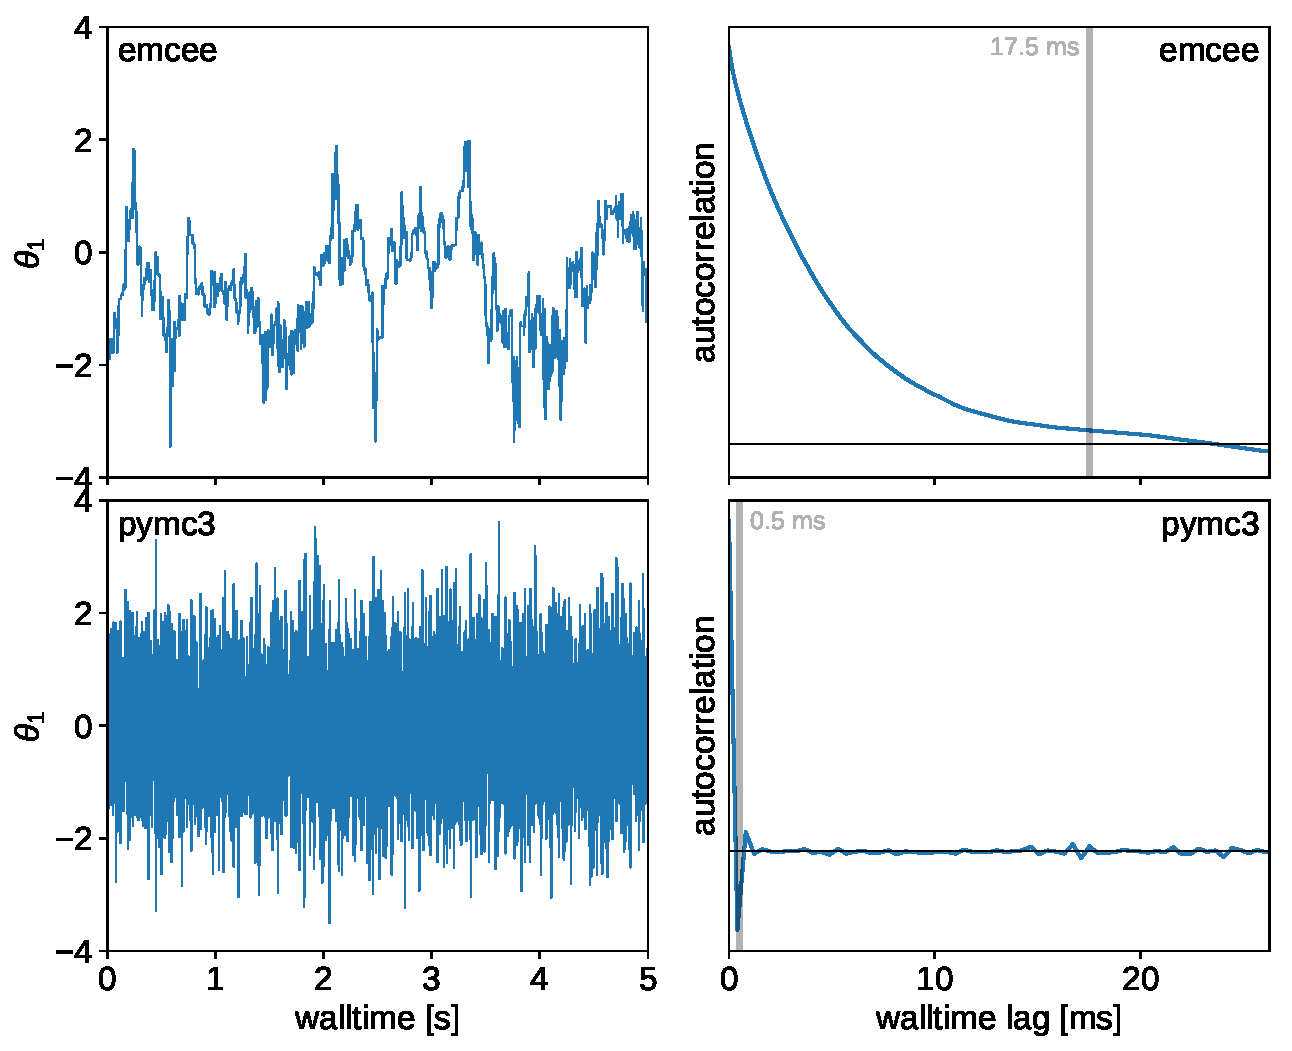
\includegraphics[width=0.8\linewidth]{figures/gaussians.pdf}
\oscaption{gaussians}{\label{fig:gaussians}
This is a figure.}
\end{centering}
\end{figure}

\section{Automatic differentiation}

The main limitation of gradient-based inference methods is that, in order to
use them, you must \emph{compute the gradients}!
The fundamental quantity of interest is the first derivative (gradient) of the
log-likelihood function (or some other goodness-of-fit function) with respect
to the parameters of the model.
In all but the simplest cases, symbolically deriving this gradient function is
tedious and error-prone.
Instead, it is generally preferable to use a method (called automatic
differentiation) that can automatically compute the exact gradients of the
model \emph{to machine precision} at compile time.
We would like to emphasize the fact that we are not talking \emph{numerical}
derivatives like finite difference methods, and there is no approximation
being made.

The basic idea behind automatic differentiation is that code is always written
as the composition of basic functions and, if we know how to differentiate the
subcomponents, then we can apply the chain rule to differentiate the larger
function.
This realization was one of the key discoveries that launched the field of
machine learning called ``deep learning'', where automatic differentiation was
given the name ``backpropagation'' (CITE).
Since then, there has been a substantial research base that has made these
methods general and computationally efficient, and from this, many open source
libraries have been released that ease the use of these methods (e.g.\
TensorFlow, PyTorch, Stan, ceres, Eigen, etc.\ CITATIONS).
Despite the existence of these projects, automatic differentiation has not
been widely adopted in the astronomical literature because there is some
learning curve associated with porting existing code bases to a new language
or framework.
Furthermore, many projects in astronomy involve fitting realistic, physically
motivated models that involve numerical solutions to differential equations
or special functions that are not natively supported by the popular automatic
differentiation frameworks.

In this paper, we demonstrate how to incorporate exoplanet-specific functions
into these frameworks and derive the functions needed to characterize
exoplanets using gradient-based methods applied to radial velocity,
astrometry, and transit datasets.
Similar derivations would certainly be tractable for microlensing, direct
imaging, and other exoplanet characterization methods, but these are left to a
future paper.

\subsection{An introduction to automatic differentiation}

% https://alexey.radul.name/ideas/2013/introduction-to-automatic-differentiation/

First of all, it's important to note that automatic differentiation is not numerical or symbolic differentiation.
It is a method for evaluating the derivatives of a function \emph{exactly} for some set of inputs, without symbolically differentiating the function.

Example:
\begin{eqnarray}
f(x) = u(x)\,v(x)
\end{eqnarray}
\begin{eqnarray}
  \frac{\dd f(x)}{\dd x} = \frac{\dd u(x)}{\dd x}\,v(x) + u(x)\,\frac{\dd v(x)}{\dd x}
\end{eqnarray}
Instead, define $x \to x + \epsilon\,\delta x$ where $\epsilon^2 = 0$.
Therefore,
\begin{eqnarray}
  u(x + \epsilon\,\delta x) = u(x) + \frac{\dd u(x)}{\dd x}\,\epsilon\,\delta x
\end{eqnarray}
This equality is exact because of our definition that $\epsilon^2 = 0$.
Therefore,
\begin{eqnarray}
f(x) + \epsilon\,\delta f &=& u(x + \epsilon\,\delta x)\,v(x + \epsilon\,\delta x) \\
&=& \left[u(x) + \frac{\dd u(x)}{\dd x}\,\epsilon\,\delta x\right]\,
    \left[v(x) + \frac{\dd v(x)}{\dd x}\,\epsilon\,\delta x\right] \\
&=& u(x)\,v(x) + \epsilon\,\left[\frac{\dd u(x)}{\dd x}\,v(x) + u(x)\,\frac{\dd v(x)}{\dd x}\right]\,\delta x
\end{eqnarray}

The basic idea is that, at its roots, a computer program is the composition of simpler operations.
If the derivatives of the simplest operations are known, the automatic differentiation library can automatically apply the chain rule to each step of the calculation to accumulate the derivative of the full program.

\subsection{Choice of modeling framework}

At present, there are many model-building libraries available in every programming language, and it is not clear which should be preferred.
Since it is a popular language for code development in astrophysics, we focus on libraries with interfaces implemented in the \python\ programming language.
The two most popular libraries for model building in \python\ are the well-supported and actively-developed packages \tensorflow\ \citep{Abadi:2016} and \pytorch\ \citep{Paszke:2017}.
Each of these libraries come with extensions that enable probabilistic modeling and gradient-based inference: \project{tensorflow-probability} \citep{Dillon:2017} and \project{Pyro} \citep{Bingham:2018}.
Both of these libraries (\tensorflow\ and \pytorch) and their inference engines are built for high performance machine learning and, while many of those features are also useful for our purposes, some of the inference goals in astrophysics are somewhat different.
For example, the primary posterior inference method implemented by these packages is variational inference \dfmtodo{(CITE)}.
\dfmtodo{We discuss the application of variational inference later in this paper}, but the primary inference method used in astrophysics is Markov chain Monte Carlo (MCMC) and the implementations of gradient-based MCMC (HMC, NUTS etc) within these packages is not as fully featured as the state-of-the-art MCMC inference packages like \pymc\ \citep{Salvatier:2016} and \stan\ \citep{Carpenter:2015, Carpenter:2017}.
So, for the purposes of this paper, we restrict our focus to \pymc\ and its modeling engine \theano\ \citep{Theano-Development-Team:2016}.

\theano\ is a model building framework for \python\ that, like \tensorflow, provides an interface for defining a computational graph that can be used to efficiently compute a model and its derivatives.
It was originally developed for deep learning, but it was adopted by the \pymc\ project and extended to support probabilistic modeling and gradient-based inference methods like Hamiltonian Monte Carlo, no U-turn sampling, and variational inference.
In our experiments, the combination of \theano\ and \pymc\ provided the best balance of modern inference features, ease of use, and computational efficiency of all the existing \python-first modeling frameworks.
The \stan\ project provides a more mature and feature-rich set of inference methods, but it is more difficult to build and debug the complicated physical models that are required by exoplanet applications using the \stan\ modeling language.
Furthermore, as discussed below, we must provide custom astronomy-specific operations as part of this library and, while it is possible to extend the \stan\ math library, we found it to be much easier to develop, test, and release the necessary features using \pymc\ and \theano.


\section{Inference methods}

Gradient-based methods can be applied to both optimization and inference tasks.
For example, the task of finding the maximum likelihood or maximum a posteriori parameters can be significantly accelerated using the gradient of the objective with respect to the model parameters.
While computing the gradient will be somewhat more expensive than computing only the value of the function, it is generally significantly more efficient than using finite difference methods.
Furthermore, since the gradients computed using automatic differentiation is exact, unlike finite difference which will suffer from numerical issues unless the step size is carefully tuned, the lack of numerical noise generally reduces the number of steps the optimizer must take before reaching the optimum.

\subsection{Optimization}

One standard inference procedure is maximum likelihood or maximum a posteriori inference by optimization.
In this case, the objective (either the likelihood or posterior function) is maximized (numerically) with respect to the input parameters.
Operations like this are commonly performed within the astronomical literature (CITE) and gradient-free methods are commonly used for this purpose (LM, NM).
These methods can work reasonably well in low dimensions when the objective is well behaved, but this performance generally degrades rapidly with the number of parameters.
In other scientific fields, gradient-based optimization is the industry standard (CITE), and these methods have been demonstrated to scale to large parameter spaces.
In astronomy, it is now common to use the \project{BFGS} optimization routine (CITE) combined with finite difference estimates of the derivatives.
These methods can be applied to larger problems, but the computational cost of evaluating the model scales with the number of dimensions and the results are generally sensitive to the choice of step size in the finite difference.
Furthermore, the numerical noise introduced by the finite difference calculations reduces the performance of the optimization routine and increases the number of model evaluations needed to reach the optimum.

In this paper, we describe the computations needed to compute the required gradients using backpropagation and these derivatives can be used to substantially improve the performance of optimization applied to exoplanet datasets.

\dfmtodo{Make an example.}

For example, we computed the number of function evaluations and total run time needed to find an estimate of the maximum likelihood parameters for a simulated radial velocity data set and compared the precision of this estimate to the \dfmtodo{true} maximum.
In this case, finite difference required \dfmtodo{how many?} as many more function evaluations.

Similarly, we compare the performance of finite difference and exoplanet for optimizing the parameters for a transiting exoplanet.
In this case... \dfmtodo{finish this}.

\subsection{Sampling}

A popular method for evaluating posterior integrals is to us Markov chain Monte Carlo (MCMC).
These methods can be substantial accelerated using gradients of the log probability with respect to the input parameters using Langevin or Hamiltonian methods.

\dfmtodo{Talk about Langevin methods? CITE things}



\subsection{Variational inference}

\section{Orbital conventions}
We choose to follow a set of orbital conventions that respects as many of the established conventions while also hewing to sensible choices of right-hand rule.

The orbit is specified in the perifocal plane $x,y,z$, technically in the $x,y$ plane, where $z=0$. Then, the choice is to decide how to rotate this coordinate frame into the observed frame, which is specified by $X,Y,Z$.

Where does the $+Z$ axis point? Towards observer. X is north, Y is east.

What is the definition of the ascending node? Where the secondary is receding from the observer.

To do this, we consider the rotation matrices
\begin{equation}
  \boldsymbol{P}_x(\phi) = \left [
  \begin{array}{ccc}
    1 & 0 & 0 \\
    0 & \cos \phi & - \sin \phi \\
    0 & \sin \phi & \cos \phi \\
    \end{array}\right]
\end{equation}
\begin{equation}
  \boldsymbol{P}_z (\phi) = \left [
  \begin{array}{ccc}
    \cos \phi & - \sin \phi & 0\\
    \sin \phi & \cos \phi & 0 \\
    0 & 0 & 1 \\
    \end{array}\right].
\end{equation}
These rotation matrices result in a \emph{clockwise} rotation of the axes, as defined using the right hand rule. This means when we look down the $z$-axis, for a positive angle $\phi$, it would be as if the $x$ and $y$ axes rotated clockwise.
In order to find out what defines counter-clockwise when considering the other rotations, we look to the right hand rule and cross products of the axes unit vectors. Since, $\hat{\bm x} \times \hat{\bm y} = \hat{\bm z}$, we know that when looking down the $z$ axis the direction of the $x$-axis towards the $y$-axis defines counter clockwise.
Similarly, we have $\hat{{\bm y}} \times \hat{{\bm z}} = \hat{{\bm x}}$, and $\hat{{\bm z}} \times \hat{{\bm x}} = \hat{{\bm y}}$.

One can see how we need to rotate by referencing Figure~\ref{fig:orbit3D}. The three rotations are (i) a rotation about the $z$-axis through an angle $\omega$ so that the $x$-axis coincides with the line of nodes at the ascending node (ii) a rotation about the $x$-axis through an angle ($-i$) so that the two planes are coincident and finally (iii) a rotation about the $z$-axis through an angle $\Omega$. As one might notice, we break from some conventions \citep[e.g.,][]{Murray:2010} in using a negative rotation for inclination, which is due to the change in how we label the ascending node. Applying these rotation matrices yields
\begin{equation}
  \left [ \begin{array}{c}
  X \\
  Y \\
  Z \\
\end{array}
  \right ] =
  \boldsymbol{P}_z (\Omega) \boldsymbol{P}_x(-i) \boldsymbol{P}_z(\omega)
  \left [
  \begin{array}{c}
  x \\
  y \\
  z \\
  \end{array}
  \right]
\end{equation}

\begin{equation}
  \begin{array}{lc}
    X =& r [ \cos \Omega (\cos \omega \cos f - \sin \omega \sin f)  - \sin \Omega  \cos i (\sin \omega \cos f + \cos \omega \sin f) ] \\
    Y =& r [ \sin \Omega (\cos \omega \cos f - \sin \omega \sin f) + \cos \Omega \cos i(\sin \omega \cos f + \cos \omega \sin f) ] \\
    Z =& - r \sin i (\sin \omega \cos f + \cos \omega \sin f).\\
\end{array}
\label{eqn:Z}
\end{equation}


Using the sum angle identities to simplify the calculations, we find
\begin{equation}
  \begin{array}{lc}
    X =& r (\cos \Omega \cos(\omega + f) - \sin(\Omega) \sin(\omega + f) \cos(i)) \\
    Y =& r (\sin \Omega \cos(\omega + f) + \cos(\Omega) \sin(\omega + f) \cos(i)) \\
    Z =& - r \sin(\omega + f) \sin(i).\\
\end{array}
\label{eqn:Z}
\end{equation}


\begin{figure}[htbp]
\begin{centering}
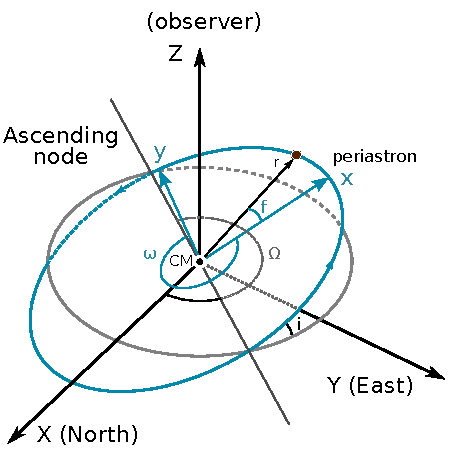
\includegraphics{figures/orbit3D.pdf}
\oscaption{orbit3D}{\figurelabel{orbit3D}
The conventions used.}
\end{centering}
\end{figure}

\section{The custom operations provided by exoplanet}

\subsection{A solver for Kepler's equation}

A key assumption that is often made when fitting exoplanets is that the
planets are orbiting the central star on independent bound Keplerian orbits
(CITE).
To compute the coordinates of a planet on its orbit, we must solve Kepler's
equation
\begin{eqnarray}
M &=& E - e\,\sin E
\end{eqnarray}
for the eccentric anomaly $E$ at fixed eccentricity $e$ and mean anomaly $M$.
This equation must be solved numerically and there is a rich literature
discussing methods for this implementation.
We have found the method from CITE to provide the right balance of numerical
stability (with a relative accuracy of about $10^{-20}$ for all values of $M$
and $e$) and computational efficiency.

As well as solving Kepler's equation, we must also efficiently evaluate the
gradients (or, more precisely, \emph{back-propagate} the gradients) of $E$
with respect to $e$ and $M$.
After solving for $E$, this can be computed efficiently and robustly using
implicit differentiation.
For numerical methods like this, it is often possible to compute the gradients
without applying automatic differentiation to the implementation directly and
that is generally preferred for the purposes of numerical stability.
In this case, the relevant gradients are
\begin{eqnarray}
\frac{\dd E}{\dd e} &=& \frac{\sin E}{1 - e\,\cos E} \\
\frac{\dd E}{\dd M} &=& \frac{1}{1 - e\,\cos E} \quad.
\end{eqnarray}

\paragraph{Implementation details}

We find that directly evaluating the true anomaly $f$
%\begin{eqnarray}
%f &=& 2\,\tan^{-1}\,left(\frac{\sqrt{1+e}}{\sqrt{1-e}}\,\tan \frac{E}{2}\right)
%\end{eqnarray}
when solving Kepler's equation is more efficient than evaluating it separately
within Theano.
This means that we must also provide a method for evaluating the derivative of
$f$ with respect to $e$ and $M$.


\subsection{Transit light curves}

Another custom operation included as part of \exoplanet\ is for calculating model light curves for the transits (and occultations) including limb-darkening and exposure time integration.
This core functionality is provided by the code \starry\ \citep{Luger:2019} \dfmtodo{cite limbdark}.
Briefly, \starry\ represents the star using a spherical harmonic representation of its surface brightness and then uses this representation to analytically integrate the surface of the star to compute the model light curve and the derivatives with respect to the physical parameters.
This algorithm is a generalization of the popular quadratic limb darkening model \citep{Mandel:2002} to a much more flexible class of stellar surface maps \dfmtodo{cite other limb darkening models}.
For our purposes, \starry's key feature is the fact that it not only computes the model light curve (as has been done previously \dfmtodo{cite}), but also the derivatives of this model with respect to the parameters of the system (the orbital parameters and the spherical harmonic coefficients).
In the case of pure limb darkening, these derivatives are calculated analytically following \dfmtodo{cite limbdark} while, in the more general case, the derivatives are accumulated using automatic differentiation in the \cpp\ code (using Eigen \dfmtodo{cite Eigen}).
\dfmtodo{Make a plot of the gradient light curves.}
This means that \starry\ can be included within the backpropagation framework needed by \exoplanet.

From an interface perspective, \starry\ is included as a set of custom \theano\ operations that compute the matrices in the \starry\ equation as a function of the sky coordinates of the bodies in the system and the spherical harmonic coefficients.
The linear algebra is performed directly in \theano.
This means that the gradients are efficiently backpropagated using the linear algebra routines provided by \theano.

\paragraph{Exposure time integration}
In many cases, the finite exposure time integration of transit light curves must be included in the model light curve in order to get correct constraints on the physical properties of the system.
\exoplanet\ includes several routines for integrating the model.
First, it includes an oversampling routine as recommended by \dfmtodo{cite kipping}, including generalizations to higher order integration schemes.
This has the benefit that it is simple to use and can generally be applied to any model light curve.
However, this method also introduces significant memory overhead because each data point requires many (at least tens) of model evaluations and these must be stored in memory for the purposes of backpropagation.

Because of this shortcoming, \exoplanet\ also implements an adaptive exposure time integration routine directly in \cpp\ that can be used for Keplerian orbits.
In this case, the time integral is performed using an adaptive Simpson's rule \dfmtodo{cite} directly in the backend, reducing the computational cost and memory overhead.
This routine works by recursively subdividing the exposure interval until a parabolic approximation to the flux in the subexposure matches the computed flux to a specified tolerance.
The derivative of this integral is accumulated using during the forward pass.

\paragraph{Performance}
As demonstrated in the papers describing this algorithm \citep{Luger:2019} \dfmtodo{cite limbdark}, the performance of the algorithms implemented in \starry\ is competitive with the other standard light curve implementations \dfmtodo{cite}.
Figure \dfmtodo{whatever} demonstrates this in the context of \exoplanet.
\dfmtodo{Make a runtime figure and explain it.}


\subsection{Scalable Gaussian Processes for time series}

\exoplanet\ also includes an implementation of scalable Gaussian Processes (GPs) using the \celerite\ algorithm \citep{Foreman-Mackey:2017}.
To make this algorithm compatible with the \theano\ automatic differentiation framework, we also derived the backpropagation functions for \celerite\ \citep{Foreman-Mackey:2018a}.
We implemented these functions in \cpp\ as a custom \theano\ operation so that they can be seamlessly integrated into a \pymc\ probabilistic model.

\celerite\ provides an algorithm for performing exact inference with GP models that scales linearly with the number of data points, instead of the typical cubic scaling.
This scaling is achieved by exploiting structure in the covariance matrix when the covariance function is restricted to be a specific stationary form, with one-dimensional inputs.
The observations can, however, be un-evenly sampled and heteroschedastic without any loss of accuracy or computational performance.
As discussed by \citet{Foreman-Mackey:2017}, this covariance function can be interpreted as the covariance generated by a mixture of stochastically-driven, damped simple harmonic oscillators, which makes this a good model for the variability of stars in the time domain.
\exoplanet\ provides an interface for constructing covariance functions that satisfy the constraints of the \celerite\ algorithm and for solving the relevant linear algebra.

This operation is useful for many exoplanet applications where the datasets are large enough that traditional GP modeling is intractable.
For example, the time series for a typical short cadence target from the \tess\ mission has a light curve with about 20,000 data points.
Evaluating a GP model on these data using high-performance general linear algebra libraries would take \dfmtodo{how long?}.

\section{Examples}



\appendix

\section{Solving Kepler's equation}

A crucial component for all of the models in this paper is an accurate and
high-performance solver for Kepler's equation
\begin{eqnarray}\eqlabel{kepler-equation}
M &=& E - e\,\sin E \quad.
\end{eqnarray}
We use the method presented by \citet{Nijenhuis:1991}.
Unlike most of the methods used in astrophysics, this algorithm \emph{is not
iterative}.
This can lead to much better compiler optimization.
Furthermore, this algorithm doesn't require the evaluation of trigonometric
functions directly.
As well as improving performance, this also increases the accuracy of the
results because it avoids catastrophic cancellations when evaluating $E - \sin
E$ and $1 - \cos E$ by evaluating these differences directly using a series
expansion.

The procedure is as follows:
\begin{enumerate}

\item Initial estimates are selected for the parameters by partitioning the
parameter space into 4 regions and applying a set of heuristics specific to
each part of parameter space.

\item This estimate is refined using either a single iteration of Halley's
second order root finding algorithm (with the sine function with its series
expansion) or a variant of the cubic approximation from \citet{Mikkola:1987}.

\item Finally, the result is updated by a single step of a high-order
generalized Newton method where the order of the method controls the target
accuracy of the method. In the \exoplanet\ implementation, we use a 4th order
update.

\end{enumerate}

The details of the implementation are exactly ported from the implementation
in \citet{Nijenhuis:1991} so we won't reproduce that here, but we did an
experiment to compare the performance and accuracy of this method to some
implementations of Kepler solvers commonly used for exoplanet fitting.
Specifically we compare to the implementations from the \batman\ transit
fitting framework \citep{Kreidberg:2015} and the \radvel\ radial velocity
fitting library \citep{Fulton:2017, Fulton:2018}.
In both cases, the solver is implemented in \project{C} and exposed to
\python\ using the \python\ \project{C}-API directly or \cython\
\citep{Behnel:2011} respectively.
Similarly, the implementation in \exoplanet\ is written in \cpp\ with \python\
bindings exposed by \theano\ \citep{Theano-Development-Team:2016}.

To test the implementation, we generated 100000 true eccentric anomalies
$E_\mathrm{true}$ uniformly distributed between $0$ and $2\,\pi$.
Then, for a range of eccentricities $e$, we computed the mean anomaly $M$ using
\eq{kepler-equation} and used each library to solve \eq{kepler-equation} for
$E_\mathrm{calc}$.
The top panel of \Figure{kepler_solver} shows the average computational cost per
solve of \eq{kepler-equation} for each library as a function of eccentricity.
The implementation of the \citet{Nijenhuis:1991} algorithm in \exoplanet\ is
more than an order of magnitude more efficient than the other methods and this
cost does not depend sensitively on the eccentricity of the orbit.
It is worth noting that both \batman\ and \exoplanet\ feature ``fused''
solvers that return both the eccentric anomaly and the true anomaly whereas
\radvel\ only computes the eccentric anomaly so there is a small amount of
computational overhead introduced into both \exoplanet\ and \batman\ when
compared to \radvel.

The bottom panel of \Figure{kepler_solver} shows the 90th percentile of the
distribution of absolute errors when comparing $E_\mathrm{true}$ and
$E_\mathrm{calc}$ for each method as a function of eccentricity.
Across all values of eccentricity, \exoplanet\ computes the eccentric anomaly
with an accuracy of better than 15 decimal places.
In some cases, the \radvel\ solver is slightly better, but at some
eccentricities, the error is more than an order of magnitude worse for
\radvel\ than for \exoplanet.
In all cases, the accuracy of the implementation from \batman\ is several
orders of magnitude worse than the other implementations.
This accuracy could be improved by decreasing the convergence tolerance in the
iterative solver at the cost of longer run times, but the current value of
$10^{-7}$ is currently hard coded\footnote{\url{%
https://github.com/lkreidberg/batman/blob/70f2c0c609124bdf4f17041bf09d5426f3c93334/c\_src/\_rsky.c\#L45}}.

\begin{figure}[htbp]
\begin{centering}
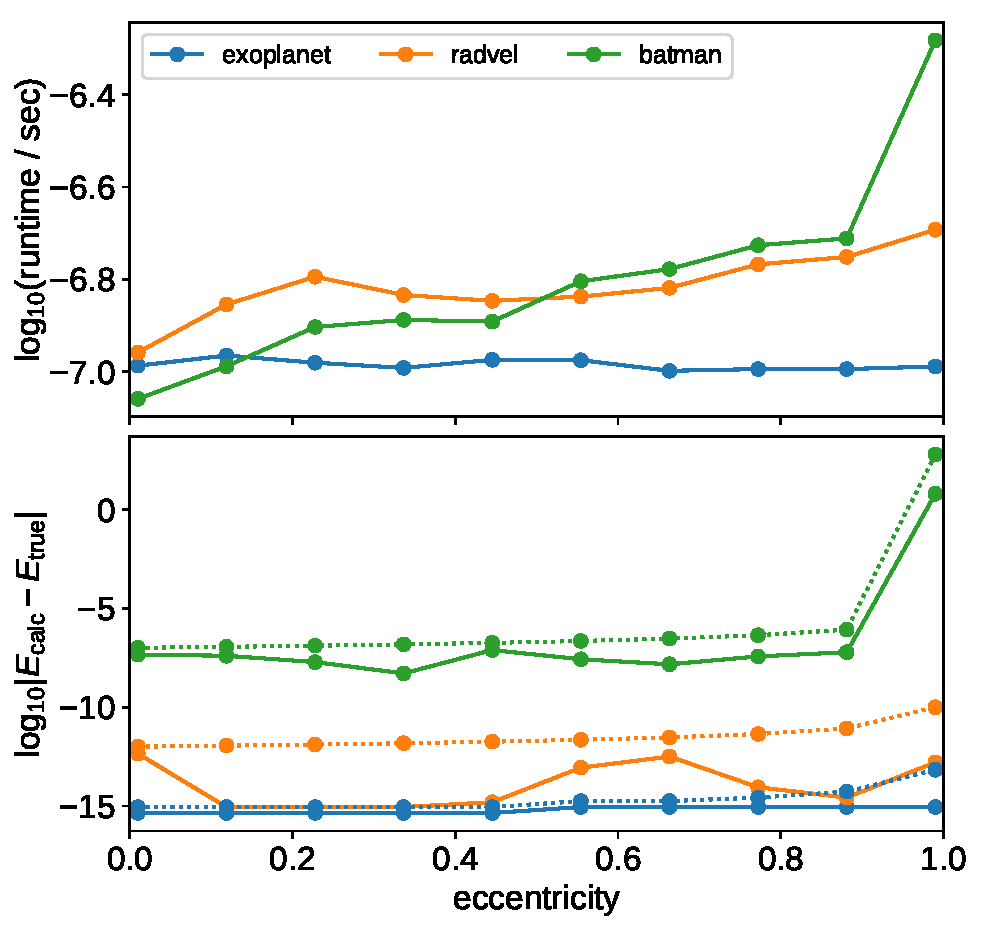
\includegraphics[width=0.8\linewidth]{figures/kepler_solver.pdf}
\oscaption{kepler_solver}{\figurelabel{kepler_solver}
The performance of the Kepler solver used by \exoplanet\ compared to
the solvers from the \radvel\ \citep{Fulton:2017, Fulton:2018} and \batman\
\citep{Kreidberg:2015} libraries.
\emph{top}: The average wall time required to solve Kepler's equation once for
the eccentric anomaly $E$ conditioned on eccentricity $e$ and mean anomaly $M$.
Smaller numbers correspond to faster solutions.
\emph{bottom}: The 90-th percentile of the absolute error of the computed
eccentric anomaly for 100000 true values of $E$ in the range $0 \le E < 2\,\pi$.
Smaller numbers correspond to more accurate solutions.}
\end{centering}
\end{figure}

\section{Contact points}

In the plane of the orbit, $S_0$, the coordinates of the orbit satisfy the
equation
\begin{eqnarray}\eqlabel{constraint0}
{({x_0} - a\,e)}^2 + \frac{{y_0}^2}{1-e^2} &=& a^2 \quad.
\end{eqnarray}
To rotate into the observing plane, we perform the following transformation
\begin{eqnarray}\eqlabel{rotation}
\bvec{x}_2 &=& R_i\,R_\omega\,\bvec{x}_0 \\
\left(\begin{array}{c}x_2\\y_2\\z_2\end{array}\right) &=&
\left(\begin{array}{ccc}
1 & 0 & 0\\
0 & \cos i & \sin i \\
0 & -\sin i & \cos i \\
\end{array}\right) \,
\left(\begin{array}{ccc}
\cos\omega & \sin\omega & 0\\
-\sin\omega & \cos\omega & 0 \\
0 & 0 & 1 \\
\end{array}\right) \,
\left(\begin{array}{c}x_0\\y_0\\0\end{array}\right) \quad.
\end{eqnarray}
In this space, the planet will transit whenever
\begin{eqnarray}
z_2 < 0 &\mathrm{and}& {x_2}^2 + {y_2}^2 < L^2
\end{eqnarray}
where $L = R_\star + R_P$.
The contact point therefore occurs when
\begin{eqnarray} \eqlabel{quad1}
\hat{x_2}^2 + \hat{y_2}^2 = L^2
\end{eqnarray}
where the hat indicates that

Using the inverse of \eq{rotation} to re-write \eq{constraint0} in terms of
$x_2$ and $y_2$, we find the following quadratic equation
\begin{eqnarray} \eqlabel{quad2}
A\,{x_2}^2 + B\,{x_2\,y_2} + C\,{y_2}^2 + D\,x_2 + E\,y_2 + F &=& 0
\end{eqnarray}
with
\begin{eqnarray}
A &=& \left(e^{2}\,\cos^{2}{\omega} - 1\right)\,\cos^{2}{i} \\
B &=& 2\,e^{2}\,\cos{i}\,\sin{\omega}\,\cos{\omega}\\
C &=& e^{2}\,\sin^{2}{\omega} - 1\\
D &=& 2\,a\,e\,\left(1-e^{2}\right)\,\cos^{2}{i}\,\cos{\omega}\\
E &=& 2\,a\,e\,\left(1-e^{2}\right)\,\sin{\omega} \cos{i}\\
F &=& a^{2}\,\left(e^{2} - 1\right)^{2}\,\cos^{2}{i}
\end{eqnarray}

The pair of quadratic equations defined by \eq{quad1} and \eq{quad2} can be
combined to give a quartic equation for $x_2$
\begin{eqnarray}
a_0 + a_1\,{x_2} + a_2\,{x_2}^2 + a_3\,{x_2}^3 + a_4\,{x_2}^4 = 0
\end{eqnarray}
where
\begin{eqnarray}
a_0 &=& \left(C L^{2} - E L + F\right) \left(C L^{2} + E L + F\right) \\
a_1 &=& - 2 \left(B E L^{2} - C D L^{2} - D F\right)\\
a_2 &=& 2 A C L^{2} + 2 A F - B^{2} L^{2} - 2 C^{2} L^{2} - 2 C F + D^{2} + E^{2}\\
a_3 &=& 2 \left(A D + B E - C D\right)\\
a_4 &=& A^{2} - 2 A C + B^{2} + C^{2}
\end{eqnarray}
which can be solved symbolically (CITE Kipping) or numerically.

\paragraph{Edge-on orbits}
For an edge-on orbit, $\cos{i} = 0$ and the contact points occur at
\begin{eqnarray}\eqlabel{edgeon1}
x_2 &=& \pm L \\
y_2 &=& 0 \quad,
\end{eqnarray}
but care must be taken when evaluating $z_2$.
To do this, we substitute \eq{edgeon1} into \eq{constraint0} to get the
following quadratic equation for $z_2$
\begin{eqnarray}
b_0 + b_1\,{z_2} + b_2\,{z_2}^2 &=& 0
\end{eqnarray}
where
\begin{eqnarray}
b_{0,\pm} &=& L^2\,(e^2\,\cos^2\omega - 1) \mp 2\,a\,e\,L\,\cos\omega\,(e^2-1) +
a^2\,{(e^2 -1)}^2 \\
b_{1,\pm} &=& -2\,a\,e\,\sin\omega\,(e^2-1) \pm 2\,e^2\,L\,\sin\omega\,\cos\omega\\
b_{2,\pm} &=& e^{2} \sin^{2}{\left (\omega \right )} - 1 \quad.
\end{eqnarray}
There are 4 solutions to this system of which we are only interested in the
ones where $z_2 < 0$ (the others are the contact points for the occultation).

\begin{figure}[htbp]
\begin{centering}
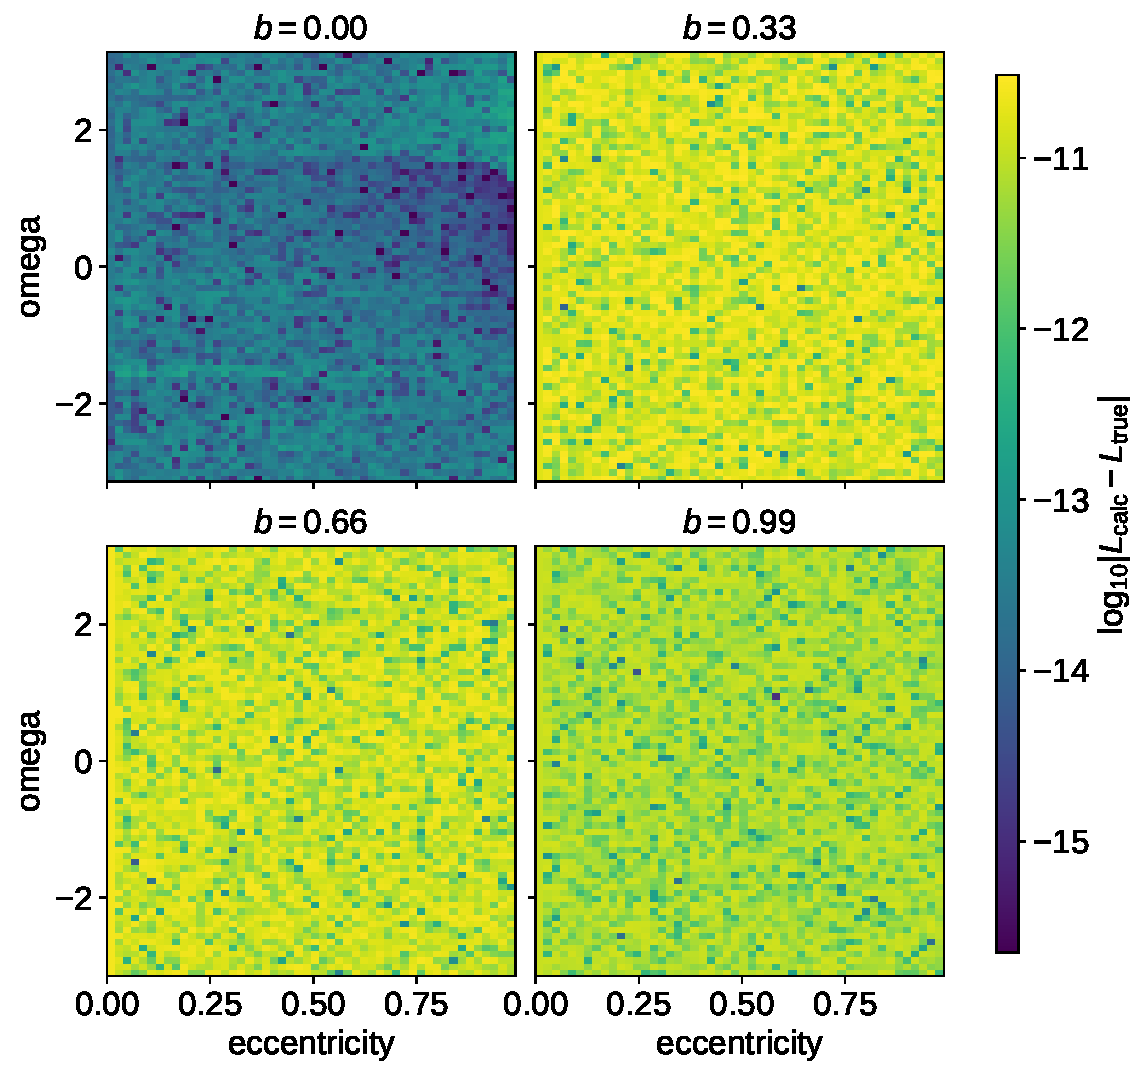
\includegraphics[width=0.8\linewidth]{figures/contact_points.pdf}
\oscaption{contact_points}{\label{fig:contact_points}
This is a figure.}
\end{centering}
\end{figure}

\section{Exposure time integration for celerite models}

In this section we give expressions for the {\it exposure-time}
integrated versions of the \celerite\ kernel and its power
spectrum.  It turns out that the time-integrated \celerite\ kernel
remains expressible as a semi-separable matrix when the exposures
do not overlap, but when exposures overlap (or for zero time
delay), the kernel no longer is semi-separable.

\paragraph{Real term}

For a real term:
\begin{equation}
%k(\tau) = a\,\exp\left(-c\,(t_i - t_j)\right)
k(\tau) = a\,\exp\left(-c\,\tau\right)
\end{equation}
where $\tau = \vert t_i-t_j \vert$.  
The integrated kernel is
\begin{proof}{celerite-integral}
k_\Delta(\tau) = \frac{2}{\left(c\,\Delta\right)^2}\,k(\tau)\,
  \begin{cases}
    \cosh(c\,\Delta) - 1 + c\,\Delta-\sinh(c\,\Delta) & \tau = 0 \\
   c(\Delta - \tau) e^{c\tau} + \cosh{(c\tau)} e^{-c(\Delta - \tau)} -1 & 0 < \tau \le \Delta \\
   \cosh(c\,\Delta) - 1  & \Delta < \tau 
    \end{cases}
%k_\Delta(\tau) = \frac{2}{\left(c\,\Delta\right)^2}\,\left[
%    \cosh(c\,\Delta) - 1
%\right]\,k(\tau)
\end{proof}
where $\Delta$ is the integration time.  Note that in the standard
use case of a single light curve with a single telescope and a
uniform exposure time, the times of each cadence will be separated 
by greater than the exposure time, and so the kernel will be
semi-separable.  However, there is a slight difference in
the implementation as the $\tau = 0$ term, which corresponds to
the diagonal of the covariance matrix, has an extra term,
$\frac{2}{(c\Delta)^2}(c\Delta-\sinh(c\Delta))$, times $k(\tau)$.
This additional term is negative, but can simply be added to the white 
noise component of the covariance matrix when implementing the \celerite\
kernel.   Given that the kernel is positive, the matrix will still
be positive definite.

Although this expression appears complicated, the Fourier transform
is less so, and is given by:
\begin{equation}
S(\omega) = \frac{ac}{\sqrt{2\pi}(c^2 + \omega^2)}  \frac{\sin^2(\tfrac{1}{2}\omega \Delta)}{(\tfrac{1}{2}\omega\Delta)^2}.
\end{equation}
Note that this is the Fourier transform of the kernel, $k(\tau)$,
multiplied by the square of a sinc function, $\mathrm{sinc}{(\omega\Delta/2)}$, 
which results from the convolution of the kernel with a top-hat 
time-integration of half-width $\Delta/2$.  Convolution in Fourier
space turns into multiplication, and the square of the sinc function
results from taking the square of the Fourier transform to obtain
the power spectrum. Also note that the since function goes to zero
when $\omega\Delta = 2\pi$, which corresponds to the twice the Nyquist frequency,
$f = \frac{2\pi}{\omega} = \Delta^{-1}$.


\paragraph{Complex term}

The result is somewhat more complicated for a complex term:
\begin{equation}
k(\tau) = (a + i\,b)\,\exp\left(-(c+i\,d)\,(t_i - t_j)\right)
\end{equation}
In this case, the integrated kernel is
\begin{equation}
k_\Delta(\tau) = (A + i\,B)\,k(\tau)
\end{equation}
where
\begin{proof}{celerite-integral}
  A = \frac{C_1\,\left[\cosh(c\,\Delta)\,\cos(d\,\Delta) - 1\right]
  - C_2\,\sinh(c\,\Delta)\,\sin(d\,\Delta)
}{\Delta^2\,(c^2 + d^2)^2}
\end{proof}
and
\begin{proof}{celerite-integral}
  B = \frac{C_2\,\left[\cosh(c\,\Delta)\,\cos(d\,\Delta) - 1\right]
  + C_1\,\sinh(c\,\Delta)\,\sin(d\,\Delta)
}{\Delta^2\,(c^2 + d^2)^2}
\end{proof}
where
\begin{eqnarray}
C_1 = 2\,(a\,c^2 - a\,d^2 + 2\,b\,c\,d)
\quad\mathrm{and}\quad
C_2 = 2\,(b\,c^2 - b\,d^2 - 2\,a\,c\,d)
\end{eqnarray}

\newpage
\acknowledgements

This research was partially conducted during the Exostar19 program at the Kavli Institute for Theoretical Physics at UC Santa Barbara, which was supported in part by the National Science Foundation under Grant No. NSF PHY-1748958.

\newpage
\bibliography{exoplanet}


\end{document}
